\documentclass[11pt, twoside, twocolumn]{article}
\usepackage[T1]{fontenc}
\usepackage[default]{gillius}
\usepackage[affil-it]{authblk}
\usepackage{graphicx}
\usepackage{natbib}
\usepackage{geometry}
\usepackage{amsmath}
\usepackage{listings}
\usepackage{lstbayes}
\usepackage{lineno}
\usepackage{subfigure}

%\linenumbers
\geometry{a4paper, total={170mm,257mm}, left=20mm, top=20mm}
\lstset{basicstyle=\ttfamily\footnotesize,breaklines=true}

\renewcommand{\baselinestretch}{1.3}

\title{Drift Diffusion Modelling}
\author[1]{Alasdair D. F. Clarke}

\affil[1]{\small University of Essex, Department of Psychology, Colchester, UK, CO4 3SQ}

\begin{document}



\twocolumn[
  \begin{@twocolumnfalse}
    \maketitle
    \begin{abstract}

\end{abstract}
  \end{@twocolumnfalse}
]




\section{Analysis Plan}

We will analyse our data by fitting a drift diffusion model (DDM) to it. This allows us to move from characterising each individual's performance in terms of accuracy and reaction time (which may be inter dependant due to speed-accuracy trade-offs) and instead measure drift rate, boundary separation and bias. 

Main paper for model is \citep{ratcliff-mckoon2008}?

\subsection{Pre-processing}

Before fitting the model to the data, we carried out the following pre-processing steps:

\begin{itemize}
\item Data from one participant were removed due to low (<15\%) accuracy for target absent trials.\\
\item Data from one participant were removed to to low (<55\%) accuracy for both target present and absent the red horizontal target condition.\\
\item Very short (<120ms) reaction times were excluded. This resulted in 20 trials (0.09\%) being removed. After removing these trials, the shortest renaming reaction time was over 200ms.
\item Similarly, very long (>10s) were removed. This totalled 12 (0.05\%) trials.\footnote{Rerun models with these criteria!}
\end{itemize}

After applying these criteria, we were left with 23,168 trials from a total of 58 observers. 

Accuracy data is shown in Figure \ref{fig:lvl3_emp}. The Bayesian $R^2 = 0.13$, 95\% HPDI = $[0.011, 0.29]$, i.e, Pearson's correlation coefficient $r = 0.36$.

\begin{figure*}
\centering
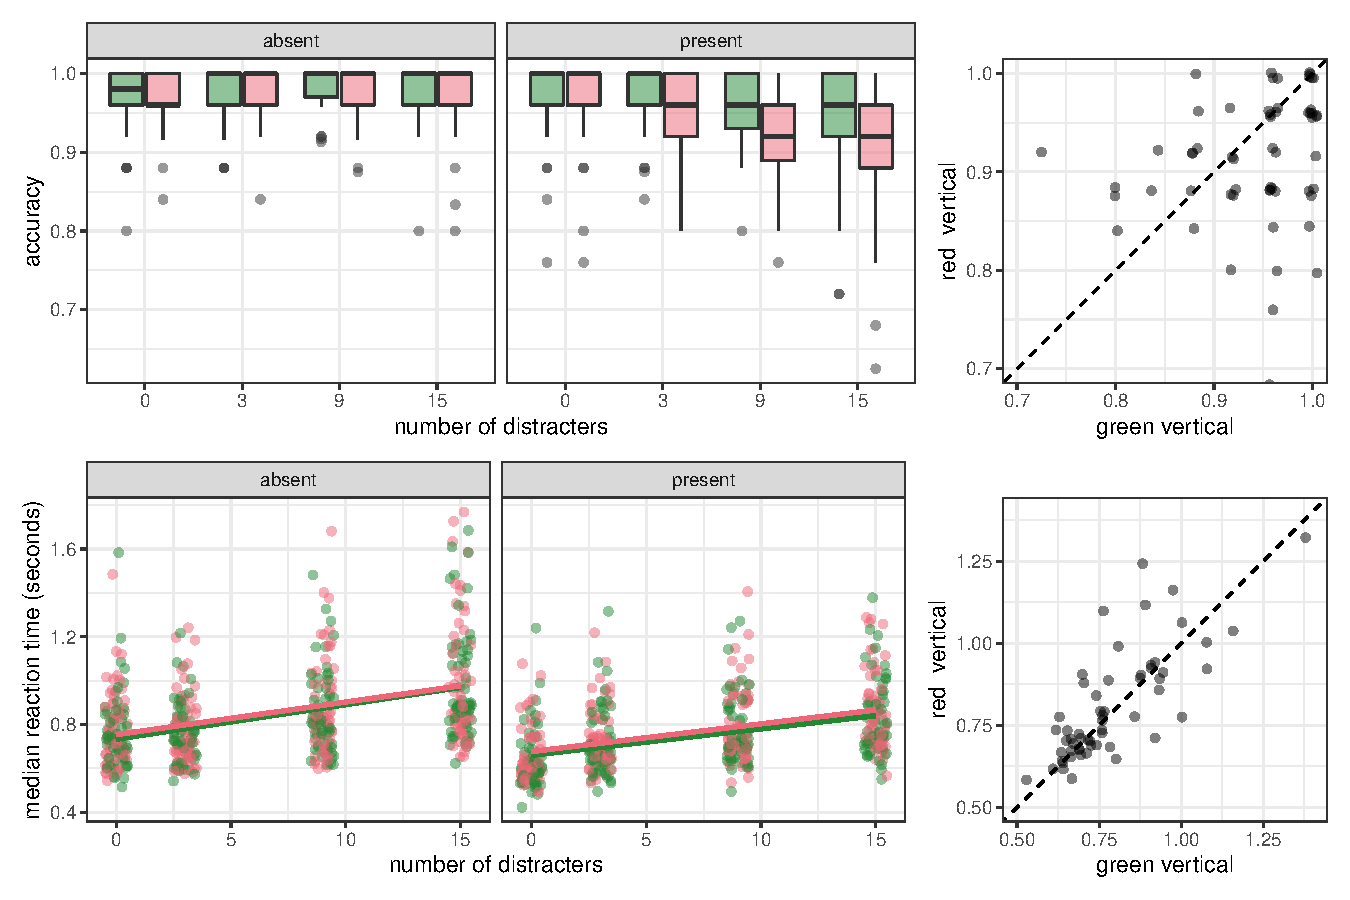
\includegraphics[width=\linewidth]{figs/exp_lvl_3_emp.pdf}
\caption{\textit{top:}Accuracy data from experiment. \textit{top right:} Accuracy data across the two condition for target absent trials with 15 distracters. Each dot represents an observer. \textit{bottom:} RT data from experiment. \textit{bottom right:} RT data across the two condition for target absent trials with 15 distracters. Each dot represents an observer.}
\label{fig:lvl3_emp}
\end{figure*}

We now look briefly at the reaction times for correct trials. 

\subsection{Modelling}

The DDM model was fit using \texttt{R} (v x.xxx) and the \texttt{brms} package (v x.xxx) with the model formula given below:

$$rt | dec \sim 0 + $$

Before fitting the model, $n_D$ was scaled to (0, 1), and the following priors were used:

More details about fitting. 

Before analysing the results, we verified that all $R\hat < 1.01$ and $n_eff>500$(???) for all parameters. 

\section{Results}

\subsection{Posterior Predictions}

First things first, we check how well the model fits the training data \ref{fig:lvl3_pred}. While we can see a good correspondance between predicted and observed RTs, the relationship with accuracy is a little less clear. This is likely to be partially due to range restriction, as we can see that both observed and predicted accuracy is close to ceiling (100\%). 

\begin{figure}
\centering
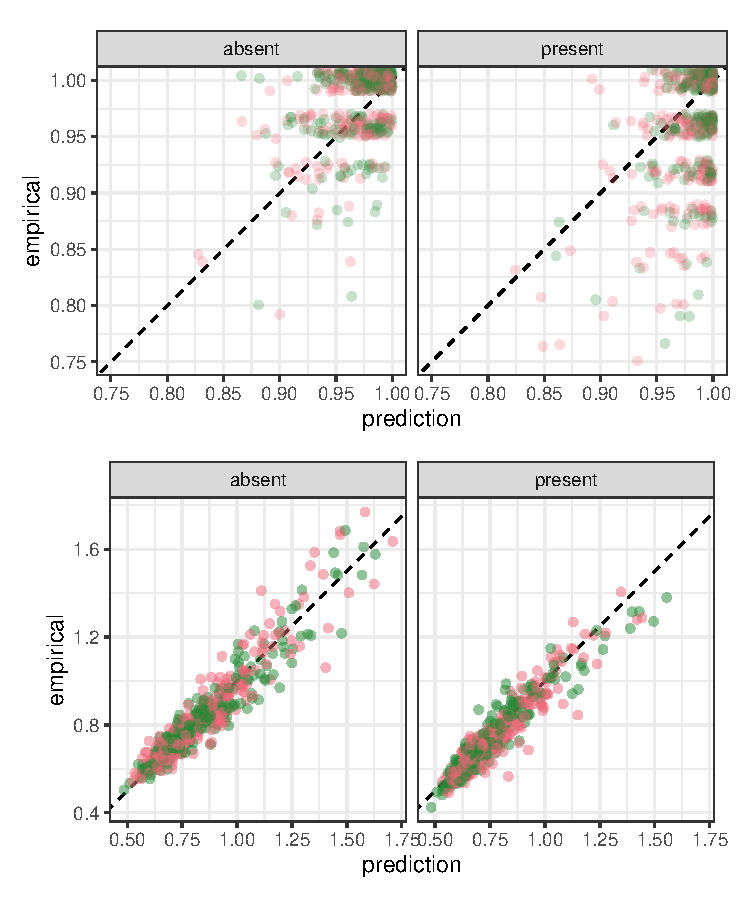
\includegraphics[width=\linewidth]{figs/exp_lvl_3_pred.pdf}
\caption{Comparisons between posterior predictions and empirical (\textit{top}) accuracies and (\textit{bottom}) RT data.}
\label{fig:lvl3_pred}
\end{figure}

\subsection{Parameter Estimates and Correlation Structure}

Posterior probability distributions, and the correlations between conditions, are shown in Figure \ref{fig:lvl3_params}. We find that increasing the number of distractors leads to increasing boundary separation, i.e., observers require more evidence to reach a decision. Reassuringly, we find correlations between parameters in the red-horizontal and green-vertical conditions. s

\begin{figure*}
\centering
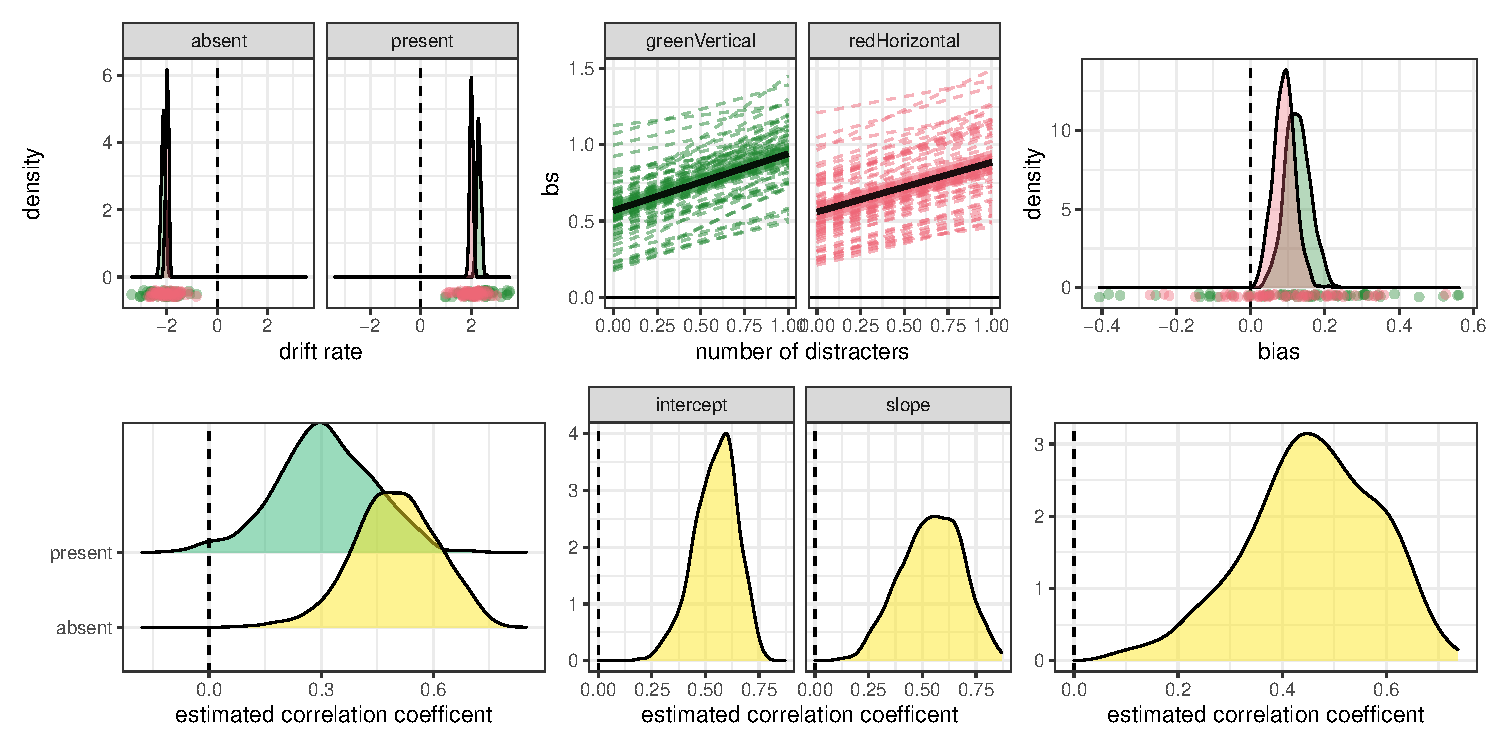
\includegraphics[width=\linewidth]{figs/exp_lvl_3_model_params.pdf}
\caption{(\textit{top}) Parameter estimates for drift rate, boundary separation and bias. (\textit{bottom}) Posterior probability distributions for the correlation between parameters in different conditions.}
\label{fig:lvl3_params}
\end{figure*}


\begin{table}[]
\begin{tabular}{rl|ccc}
\textit{param}               &                & \textit{lower} & \textit{median} & \textit{upper} \\
\hline
drift rate          & target absent  & 0.30  & 0.50   & 0.71  \\
drift rate          & target present & 0.08  & 0.31   & 0.58  \\
boundary sep. & intercept      & 0.56  & 0.36   & 0.73  \\
boundary sep. & slope          & 0.28  & 0.55   & 0.81  \\
bias                &                & 0.20  & 0.46   & 0.67  \\
\end{tabular}
\caption{Median and $95\%$ HPDIs for the correlations in parameter estimates between the two conditions.}
\label{tab:lvl3}
\end{table}


\section{Discussion}




\section{Author Contributions}


\section{Acknowledgements}

This research was supported by the Economic and Social Research Council (ESRC, ES/S016120/1). The authors would like to thank all researchers who share their data on OSF. 

\small
\bibliographystyle{apalike} 
\bibliography{literature}
\normalsize




\end{document}

